\documentclass[12pt,a4paper]{ctexart}
\usepackage{amsmath,amssymb}
\usepackage{booktabs}
\usepackage{array}
\usepackage{tabularx}
\usepackage{geometry}
\usepackage{graphicx}
\usepackage{float}
\geometry{left=2.4cm,right=2.4cm,top=2.5cm,bottom=2.5cm}
\setlength{\parindent}{2em}
\renewcommand{\arraystretch}{1.15}

\newcommand{\norm}[1]{\left\lVert #1 \right\rVert}
\newcolumntype{Y}{>{\raggedright\arraybackslash}X}

\begin{document}
\thispagestyle{empty}

\begin{center}
    {\zihao{2}\bfseries 实验报告}

    \vspace{0.7em}
    {\zihao{4}数值分析实验二}

    \vspace{1em}
    姓名：蔡斌 \qquad 学号：1024001338 \qquad 班级：\mbox{数学jd2401}
\end{center}

\section{实验目的}

\begin{enumerate}
    \item 掌握利用 Hermite 插值构造同时满足函数值与导数值条件的插值多项式；
    \item 掌握 Hermite 插值余项公式，并据此估计理论误差上限；
    \item 结合数值作图与牛顿法，估计插值误差函数的实际最大值。
\end{enumerate}

\section{实验题目}

在区间 $[-1,1]$ 上，已知函数 $f(x)=e^x$ 在节点
\[
x_0=-1,\qquad x_1=0,\qquad x_2=1
\]
处的函数值和导数值如下：
\begin{table}[H]
    \centering
    \begin{tabular}{cccc}
        \toprule
        $i$ & 0 & 1 & 2 \\
        \midrule
        $x_i$ & -1 & 0 & 1 \\
        $f(x_i)$ & $e^{-1}$ & 1 & $e$ \\
        $f'(x_i)$ & $e^{-1}$ & 1 & $e$ \\
        \bottomrule
    \end{tabular}
\end{table}

要求完成以下内容：
\begin{enumerate}
    \item 给出 Hermite 插值多项式 $H_5(x)$；
    \item 估计理论误差上限；
    \item 估计实际误差上限：作出误差函数 $\varepsilon(x)=e^x-H_5(x)$ 的图像，并用牛顿法求其极大值。
\end{enumerate}

\section{实验原理}

\subsection{Hermite 插值原理}

当已知若干节点处的函数值和导数值时，可以构造 Hermite 插值多项式。对于本题，由于有 $3$ 个节点，每个节点同时给出函数值与一阶导数值，因此可构造一个不超过 $5$ 次的 Hermite 插值多项式 $H_5(x)$，使其满足
\[
H_5(x_i)=f(x_i),\qquad H_5'(x_i)=f'(x_i),\qquad i=0,1,2.
\]

\subsection{误差公式}

Hermite 插值的余项为
\[
R_5(x)=f(x)-H_5(x)=\frac{f^{(6)}(\xi_x)}{6!}(x+1)^2x^2(x-1)^2,\qquad \xi_x\in(-1,1).
\]
由于本题 $f(x)=e^x$，故
\[
f^{(6)}(x)=e^x.
\]
因此可以利用 $e^x$ 在区间上的最大值估计理论误差上限。

\subsection{牛顿法原理}

为了估计实际误差上限，需要求误差函数
\[
\varepsilon(x)=e^x-H_5(x)
\]
在区间 $[-1,1]$ 上的最大值。极值点满足
\[
\varepsilon'(x)=0.
\]
用牛顿法求根时，迭代格式为
\[
x_{k+1}=x_k-\frac{\varepsilon'(x_k)}{\varepsilon''(x_k)}.
\]

\section{实验步骤}

\begin{enumerate}
    \item 采用 Hermite 重节点法，取节点序列 $-1,-1,0,0,1,1$，构造插值多项式；
    \item 写出余项公式，并在 $[-1,1]$ 上估计理论误差上限；
    \item 利用 MATLAB 绘制误差函数 $\varepsilon(x)=e^x-H_5(x)$ 的图像；
    \item 在区间 $(-1,0)$ 与 $(0,1)$ 内分别选取初值，利用牛顿法求解 $\varepsilon'(x)=0$；
    \item 比较各极值点处的误差函数值，得到实际误差上限。
\end{enumerate}

\section{实验结果}

\subsection{Hermite 插值多项式}

取重节点
\[
z_0=z_1=-1,\qquad z_2=z_3=0,\qquad z_4=z_5=1.
\]
对应的主要差商为
\[
\begin{aligned}
&f[z_0]=e^{-1},\qquad f[z_0,z_1]=e^{-1},\\
&f[z_0,z_1,z_2]=1-2e^{-1},\\
&f[z_0,z_1,z_2,z_3]=-1+3e^{-1},\\
&f[z_0,z_1,z_2,z_3,z_4]=\frac{e^2-7}{4e},\\
&f[z_0,z_1,z_2,z_3,z_4,z_5]=1+e^{-1}-\frac{e}{2}.
\end{aligned}
\]

因此 Hermite 插值多项式的 Newton 形式为
\[
\begin{aligned}
H_5(x)=&\,e^{-1}+e^{-1}(x+1)+(1-2e^{-1})(x+1)^2 \\
&+(-1+3e^{-1})(x+1)^2x \\
&+\frac{e^2-7}{4e}(x+1)^2x^2 \\
&+\left(1+e^{-1}-\frac{e}{2}\right)(x+1)^2x^2(x-1).
\end{aligned}
\]

将其展开，得
\[
\begin{aligned}
H_5(x)=&\left(1+e^{-1}-\frac{e}{2}\right)x^5
 +\left(1-\frac{3}{4e}-\frac{e}{4}\right)x^4\\
&+\left(e-2-\frac{3}{2e}\right)x^3
+\left(-2+\frac{5}{4e}+\frac{3e}{4}\right)x^2+x+1.
\end{aligned}
\]

\subsection{理论误差上限}

由余项公式
\[
R_5(x)=\frac{e^{\xi_x}}{720}(x+1)^2x^2(x-1)^2,
\qquad \xi_x\in(-1,1),
\]
并且在 $[-1,1]$ 上有
\[
e^{\xi_x}\le e.
\]

令
\[
\omega(x)=(x+1)^2x^2(x-1)^2=x^2(1-x^2)^2,
\]
则
\[
\omega'(x)=2x(x-1)(x+1)(3x^2-1).
\]
因此在区间 $[-1,1]$ 内，
\[
\omega(x)
\]
的极值点为
\[
x=0,\ \pm 1,\ \pm \frac{1}{\sqrt{3}}.
\]
代入可得
\[
\max_{x\in[-1,1]}\omega(x)=\omega\!\left(\pm\frac{1}{\sqrt{3}}\right)=\frac{4}{27}.
\]

所以理论误差上限为
\[
\max_{x\in[-1,1]}|R_5(x)|
\le
\frac{e}{720}\cdot \frac{4}{27}
=\frac{e}{4860}
\approx 5.59317\times 10^{-4}.
\]

\subsection{实际误差上限}

令
\[
\varepsilon(x)=e^x-H_5(x).
\]
由图像可以看出，$\varepsilon(x)$ 在 $(-1,0)$ 和 $(0,1)$ 内各有一个局部极大点，而在 $x=-1,0,1$ 处均为零。MATLAB 绘图结果如图 \ref{fig:error} 所示。

\begin{figure}[H]
    \centering
    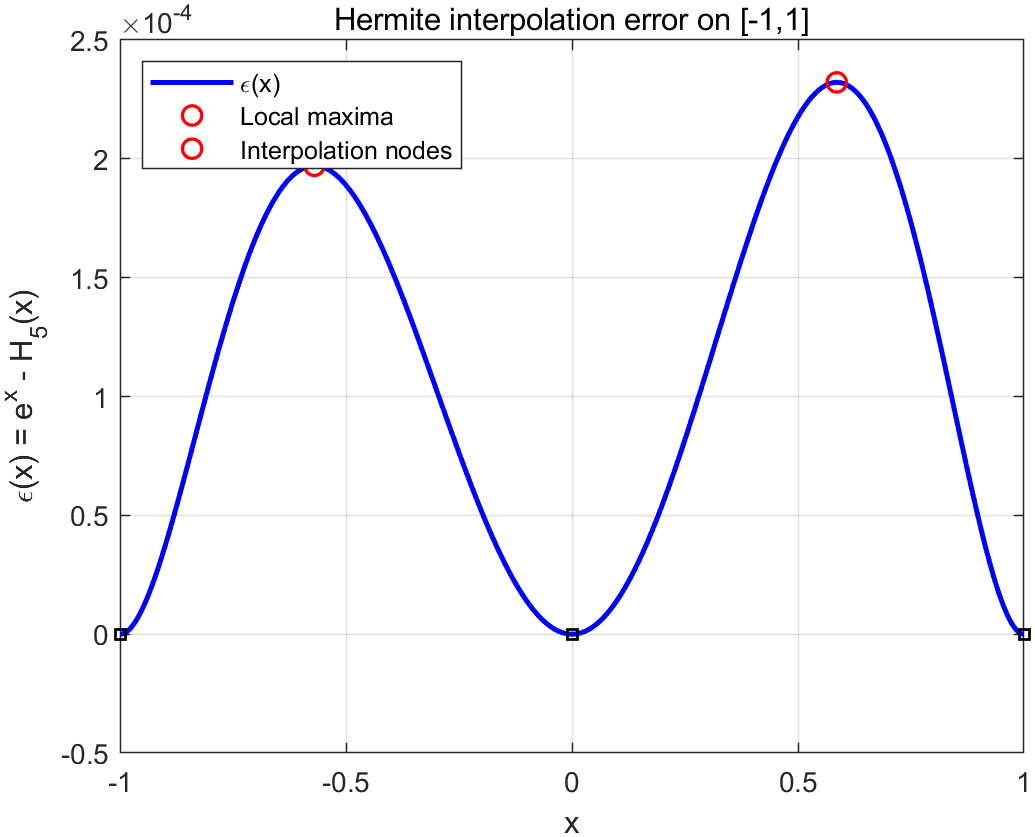
\includegraphics[width=0.78\textwidth]{epsilon_plot.png}
    \caption{误差函数 $\varepsilon(x)=e^x-H_5(x)$ 的图像}
    \label{fig:error}
\end{figure}

对
\[
\varepsilon'(x)=0
\]
分别取初值 $x_0=-0.6$ 和 $x_0=0.6$ 用牛顿法迭代，得到
\[
x_-\approx -0.569888386850,\qquad
x_+\approx 0.585678216873.
\]
对应的误差函数值为
\[
\varepsilon(x_-)\approx 1.970593508\times 10^{-4},
\]
\[
\varepsilon(x_+)\approx 2.321658302\times 10^{-4}.
\]

由于
\[
\varepsilon(x_+)>\varepsilon(x_-),
\]
因此实际误差上限为
\[
\max_{x\in[-1,1]}\varepsilon(x)
\approx 2.321658302\times 10^{-4},
\]
其达到位置约为
\[
x\approx 0.585678216873.
\]

\section{结果分析}

理论误差上限为
\[
5.59317\times 10^{-4},
\]
而实际误差上限约为
\[
2.32166\times 10^{-4}.
\]
二者比较可见，实际最大误差约为理论上界的
\[
\frac{2.32166\times 10^{-4}}{5.59317\times 10^{-4}}
\approx 0.4151.
\]

这说明 Hermite 余项给出的理论上界是有效的，但它只是保守估计，并不一定紧。对于本题，插值误差整体较小，说明在区间 $[-1,1]$ 上利用三个节点及其导数值构造出的五次 Hermite 插值多项式，对 $e^x$ 具有较好的逼近效果。

从误差图像还可以看出，误差函数在插值节点 $x=-1,0,1$ 处为零，这是 Hermite 插值满足函数值和导数值条件的直接体现；同时，由于右侧区间内 $e^x$ 增长更快，故在 $(0,1)$ 内取得了全区间最大的插值误差。

\section{实验结论}

\begin{enumerate}
    \item 已构造出函数 $f(x)=e^x$ 在节点 $-1,0,1$ 处的一次导数 Hermite 插值多项式 $H_5(x)$；
    \item 利用余项公式可得理论误差上限为
    \[
    \frac{e}{4860}\approx 5.59317\times 10^{-4};
    \]
    \item 利用 MATLAB 作图并结合牛顿法求解 $\varepsilon'(x)=0$，得到实际误差上限约为
    \[
    2.32166\times 10^{-4};
    \]
    \item 实际误差明显小于理论误差上限，表明 Hermite 插值对本题具有较好的逼近精度，理论上界能够正确反映误差范围。
\end{enumerate}

\appendix
\pagestyle{plain}
\markboth{}{}

\clearpage
\section*{附录：MATLAB 牛顿法迭代结果}

以 $x_0=-0.6$ 和 $x_0=0.6$ 为初值时，牛顿法分别在 $3$ 次迭代内收敛到极大点附近：
\[
-0.6\to -0.570318274474\to -0.569888529722\to -0.569888386850,
\]
\[
0.6\to 0.585845286167\to 0.585678243821\to 0.585678216873.
\]

由此可见，牛顿法对本题误差函数导数的求根具有较快的收敛速度。

\end{document}
